% Created 2019-01-25 Fri 10:46
\documentclass[11pt]{article}
\usepackage[utf8]{inputenc}
\usepackage[T1]{fontenc}
\usepackage{fixltx2e}
\usepackage{graphicx}
\usepackage{longtable}
\usepackage{float}
\usepackage{wrapfig}
\usepackage{rotating}
\usepackage[normalem]{ulem}
\usepackage{amsmath}
\usepackage{textcomp}
\usepackage{marvosym}
\usepackage{wasysym}
\usepackage{amssymb}
\usepackage{hyperref}
\tolerance=1000
\usepackage{color}
\usepackage{minted}
\usepackage[margin=2cm]{geometry}
\date{}
\title{Strobe Light Melody Maker}
\begin{document}

\maketitle
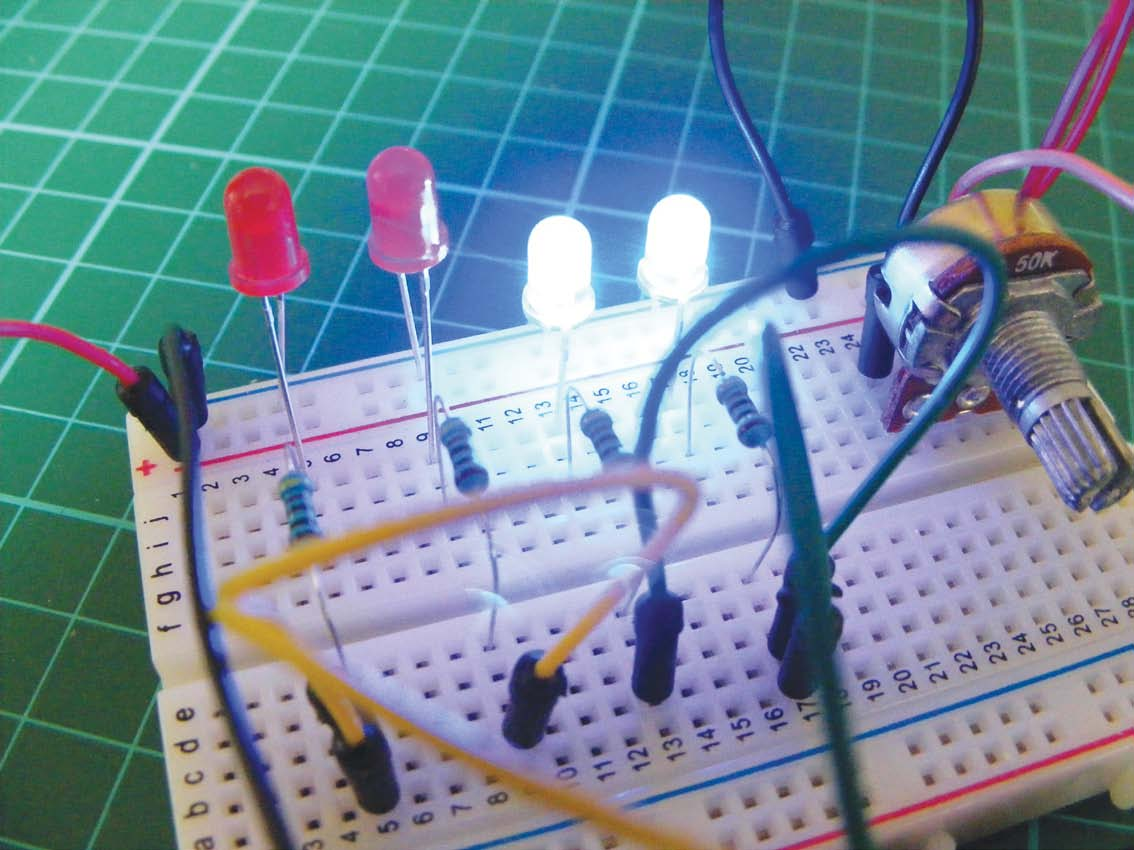
\includegraphics[width=.9\linewidth]{./arduino-images-044.png}

\section{Setup}
\label{sec-1}

First you will need to download, unzip, and install the Arduino Integrated Development Environment (IDE) from
\url{https://www.arduino.cc/en/Main/Donate} (does not need admin privileges).

\section{How it works}
\label{sec-2}

The Arduino melody project uses a piezo buzzer to create frequencies (i.e. beeps) that resemble recognizable notes. You
use the Arduino IDE to give the order, rate, and duration of the notes to play a specific tune.  Piezos are inexpensive
buzzers often used in small toys. A piezo element without its plastic housing looks like a gold metallic disc with
connected positive (typically red) and negative (typically black) wires.  A piezo is capable only of making a clicking
sound, which we create by applying voltage. We can make recognizable notes by getting the piezo to click hundreds of
times a second at a particular frequency, so first we need to know the frequency of the different tones we want. The
table below shows the notes and their corresponding frequencies.


Middle C notes (A = 440 Hz):

\begin{center}
\begin{tabular}{lrrr}
Note & Frequency (Hz) & Period (microseconds) & Time High\\
\hline
C & 261 & 3830 & 1915\\
C\# & 277 & 3610 & 1805\\
D & 294 & 3400 & 1700\\
Eb & 311 & 3216 & 1608\\
E & 329 & 3038 & 1519\\
F & 349 & 2864 & 1432\\
F\# & 370 & 2702 & 1351\\
G & 392 & 2550 & 1275\\
G\# & 415 & 2410 & 1205\\
A & 440 & 2272 & 1136\\
Bb & 466 & 2146 & 1073\\
B & 493 & 2028 & 1014\\
C & 523 & 1912 & 956\\
\end{tabular}
\end{center}


Lower Octave:

\begin{center}
\begin{tabular}{lrrr}
Note & Frequency (Hz) & Period (microseconds) & Time High\\
\hline
C & 131 & 7632 & 3816\\
C\# & 139 & 7192 & 3596\\
D & 147 & 6802 & 3401\\
Eb & 156 & 6410 & 3205\\
E & 165 & 6060 & 3030\\
F & 175 & 5714 & 2857\\
F\# & 185 & 5405 & 2702\\
G & 196 & 5102 & 2551\\
G\# & 208 & 4808 & 2404\\
A & 220 & 9088 & 2272\\
Bb & 233 & 4292 & 2146\\
B & 247 & 4050 & 2025\\
C & 261 & 3830 & 1915\\
\end{tabular}
\end{center}


Higher Octave:

\begin{center}
\begin{tabular}{lrrr}
Note & Frequency (Hz) & Period (microseconds) & Time High\\
\hline
C & 523 & 1912 & 956\\
C\# & 554 & 1804 & 902\\
D & 587 & 1702 & 851\\
Eb & 622 & 1608 & 804\\
E & 659 & 1518 & 759\\
F & 698 & 1432 & 716\\
F\# & 740 & 1352 & 676\\
G & 784 & 1276 & 638\\
G\# & 831 & 1204 & 602\\
A & 880 & 1136 & 568\\
Bb & 932 & 1072 & 536\\
B & 988 & 1012 & 506\\
C & 1047 & 946 & 478\\
\end{tabular}
\end{center}

Period is the duration of time, in microseconds, at which the frequency is created. We halve this number to get the
\texttt{time\_high} value (from the equation below), which is used in the code to create the note. The code sends a square wave
of the appropriate frequency to the piezo, generating the corresponding tone. The tones are calculated through the
following equation:

\begin{equation}
time\_high = \frac{period}{2} \\ &
           = \frac{1}{(2 * frequency)}
\end{equation}

Turning the potentiometer up or down causes the pin connected to it to read a different value, which we use to set the
overall tempo of the melody. We then use the calculated tempo to play the melody, and each time a specific note is
played, the corresponding LED will light up.

\section{Building The Circuit}
\label{sec-3}

The schematics for the circuits you will be building is below.

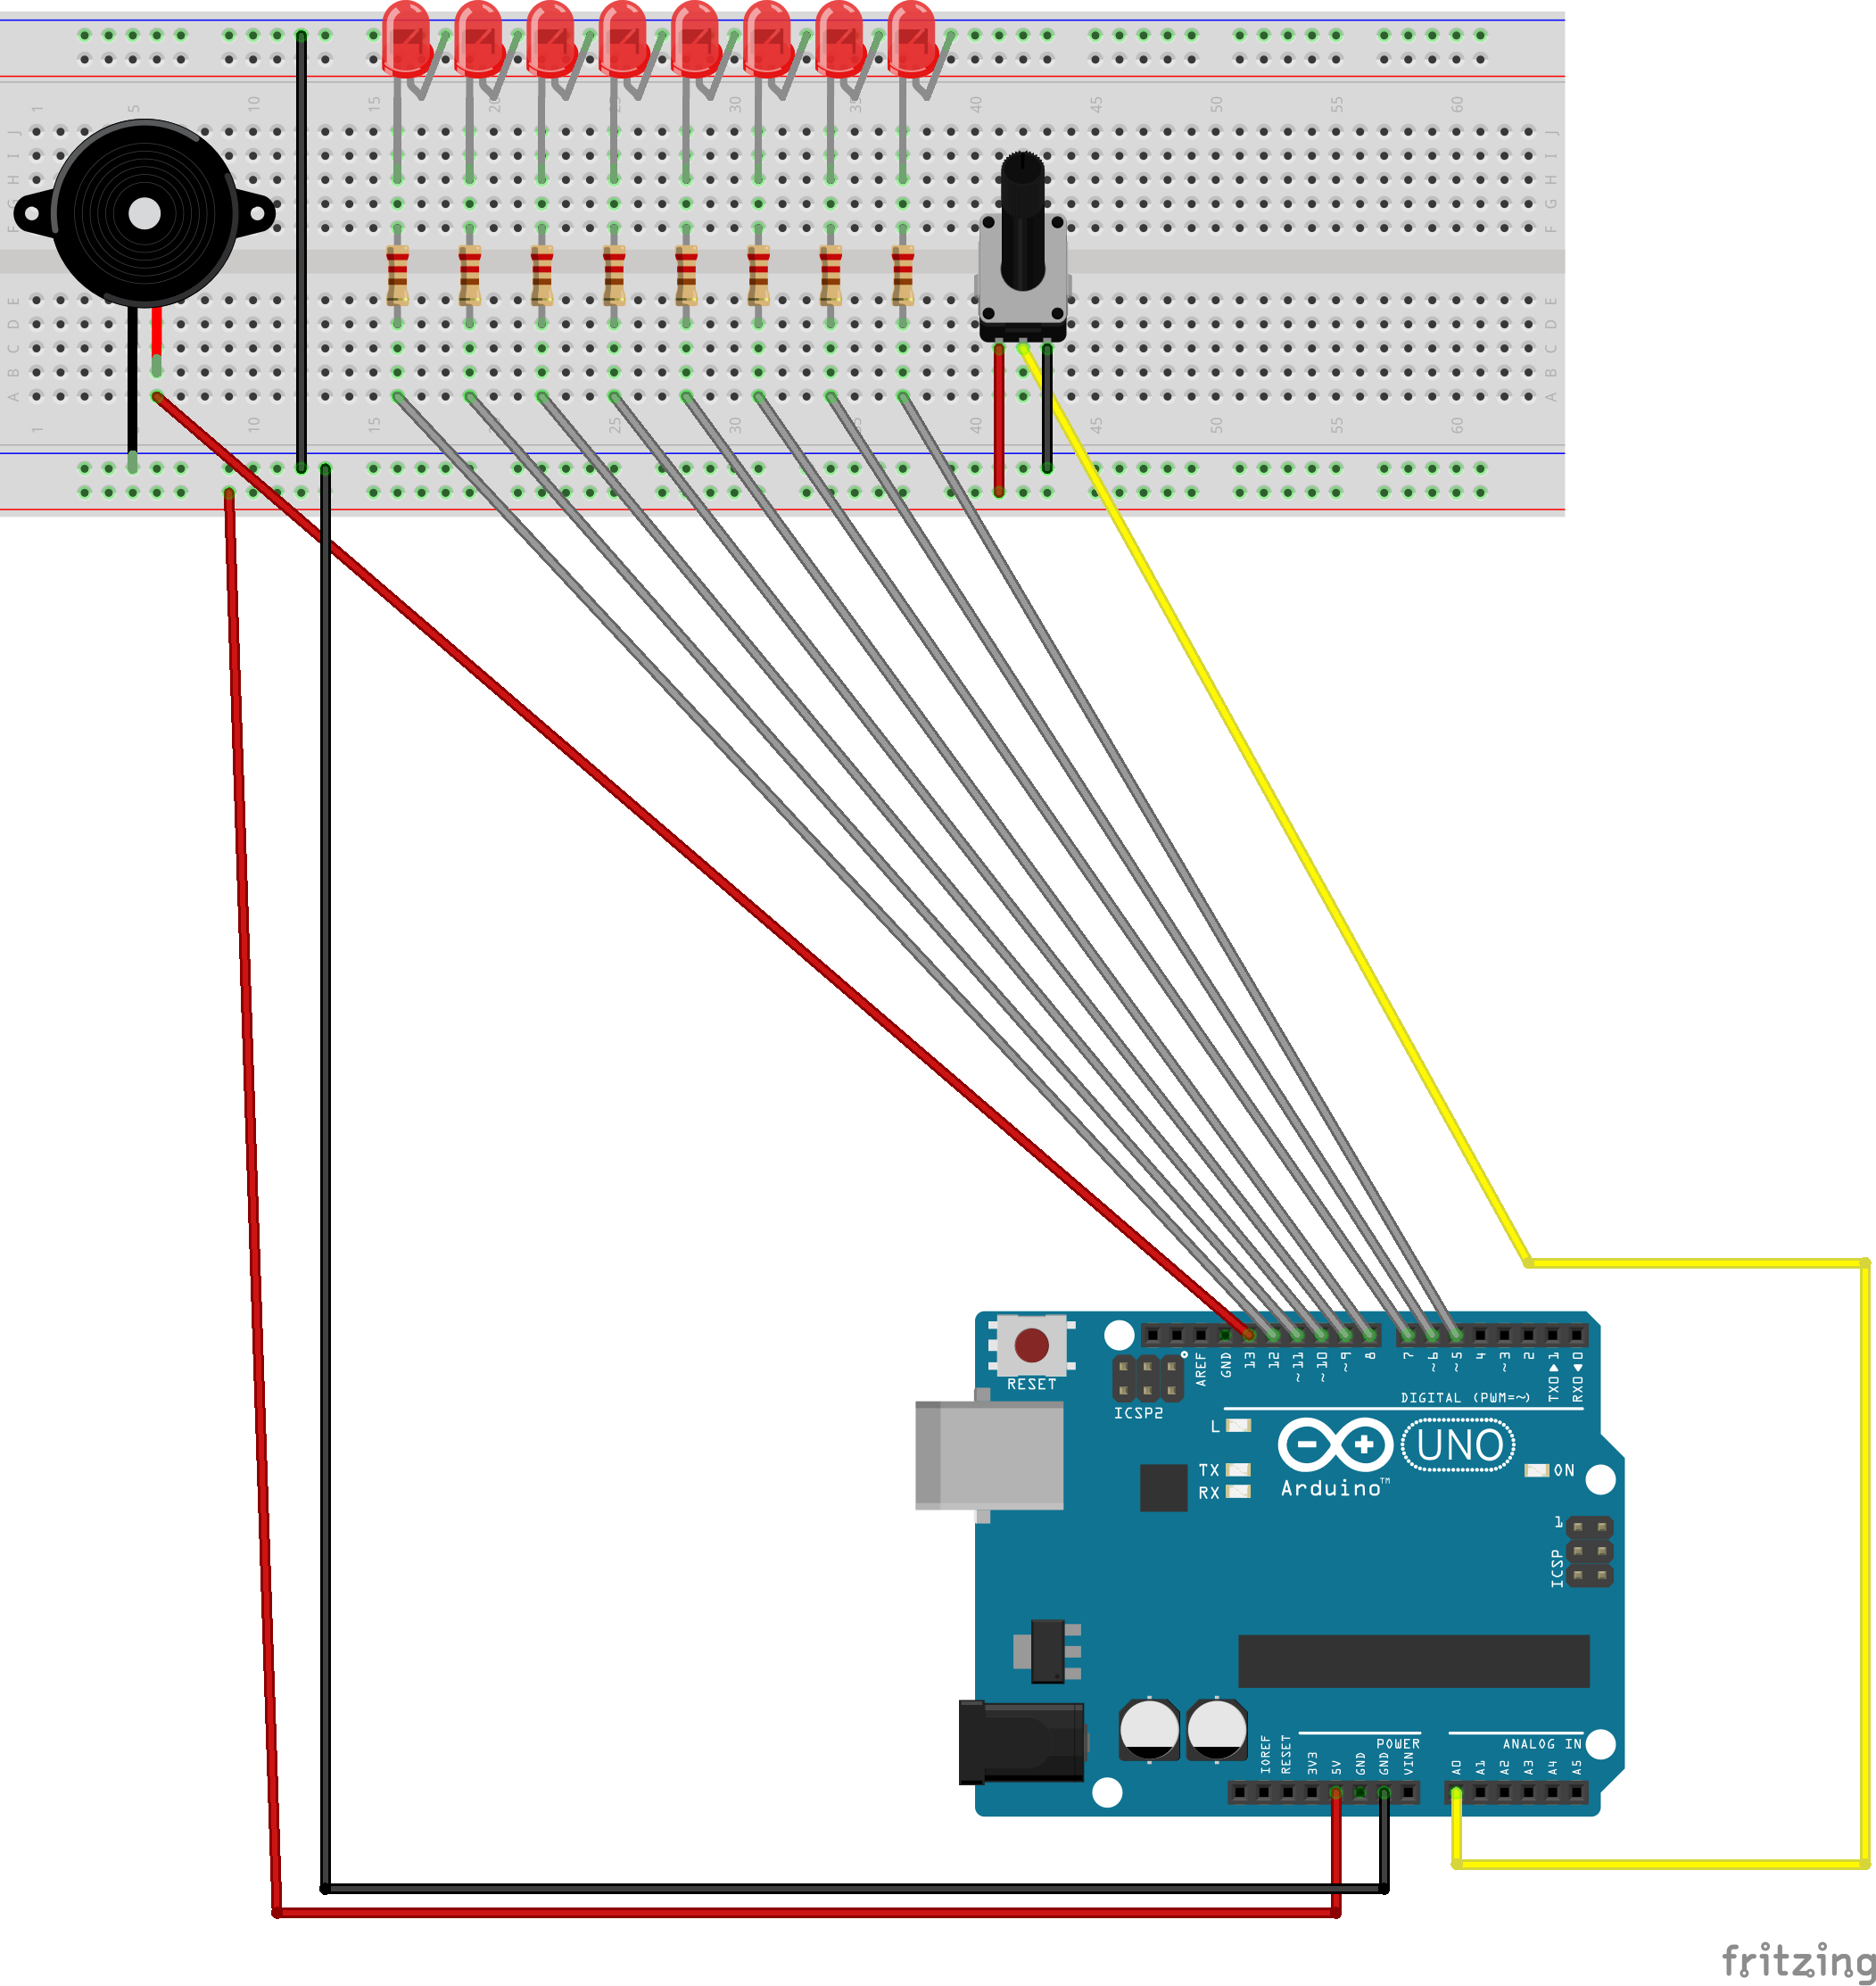
\includegraphics[width=.9\linewidth]{./exp5-strobe-melody_bb.png}

\section{Programming the Arduino}
\label{sec-4}

The base code for programming the Arduino is provided. Using the Arduino IDE, open the \texttt{.ino} file.

The IDE allows you to do 4 things: edit the code, verify the code is correct (i.e. does not contain syntax
errors), upload the code to the Arduino, and view the diagnostic output of things as they run on the Arduino.

Uploading to the Arduino is easy! Just click the Upload arrow in the IDE.

\section{The Melody Code}
\label{sec-5}

In the code, we have divided the overall task of "read a note from the melody and play it on the buzzer" into a set of
much smaller subtasks. Each chunk is called a function, and is responsible for doing one small part of the overall
task. The tasks are:

\begin{enumerate}
\item Read the value of the potentiometer and determine the tempo
\item Find the correct LED to light up based on the current note in the melody
\item Play the corresponding tone for the current note in the melody.
\end{enumerate}

\subsection{Technical details}
\label{sec-5-1}

In order to use the piezoelectric buzzer to play a tune we need to tell it 4 things:

\begin{enumerate}
\item How many notes are in the melody. This is the \texttt{MELODY\_LENGTH} constant.
\item The names of the musical notes in the melody. This is the \texttt{notes} array in the code.
\item How long to play each musical note for in the melody (in terms of beats). This is the \texttt{beats} array in the
code. Assuming the time signature is \texttt{4/4}, then a quarter note should have a value of 1, and a whole note should
have a value of 4.
\item How fast to play the melody. We use a potentiometer to make the melody play faster/slower depending on the value
read.
\end{enumerate}

If you want to switch between playing the two sample melodies, just change the 1 to a 0 and vice versa on the lines with
the \texttt{=\#if=} and \texttt{=\#elif=}.

\section{Extending The Code}
\label{sec-6}

Once you have gotten the sample melodies to play, try going online to find a short melody you like (such as one from a
video game or movie), and see if you can figure out the notes and durations and get it to play!

\begin{itemize}
\item You will probably have to change the scale from the Middle C scale used by the default melody to one that contains all
the notes of the melody you want to play (the frequencies for the octave above and below the Middle C scale are
included above).

\item If you change the scale, and it contains notes like 'B' and 'Bb' (B-flat), how can you change the code to distinguish
them?
\end{itemize}
% Emacs 25.2.2 (Org mode 8.2.10)
\end{document}
